\apendice{Documentación de usuario}

\section{Requisitos \textit{software} y \textit{hardware} para ejecutar el proyecto.}

En este caso, para la realización del proyecto, se ha empleado Python a nivel de CPU (con el ordenador personal) como herramienta principal para el desarrollo y ejecución de código, aunque, como ya se ha comentado en el apartado de ``\textit{Conclusiones}'' de la memoria, lo ideal hubiera sido usar un GPU.

La instalación de Python se puede realizar de diversas maneras. En esta ocasión, se ha hecho a partir de anaconda, una distribución de Python con una variedad de paquetes científicos.

\subsection{Pasos para la instalación de anaconda y Python}

\subsubsection{1. Descarga de anaconda en el sistema}
    
    La instalación de anaconda es bastante simple e intuitiva. A continuación, se hace una breve descripción para su correcta instalación.

    En primer lugar, se accede a la página oficial de descargas de anaconda \footnote{\url{https://www.anaconda.com/download/success}}. Una vez dentro, se elige la mejor opción de descarga para el usuario en concreto según su sistema operativo, tal y como se muestra en la figura \ref{fig:sistema_operativo_anaconda}. En este caso se ha descargado la versión para Windows.
    
    \begin{figure}[h]
        \centering
        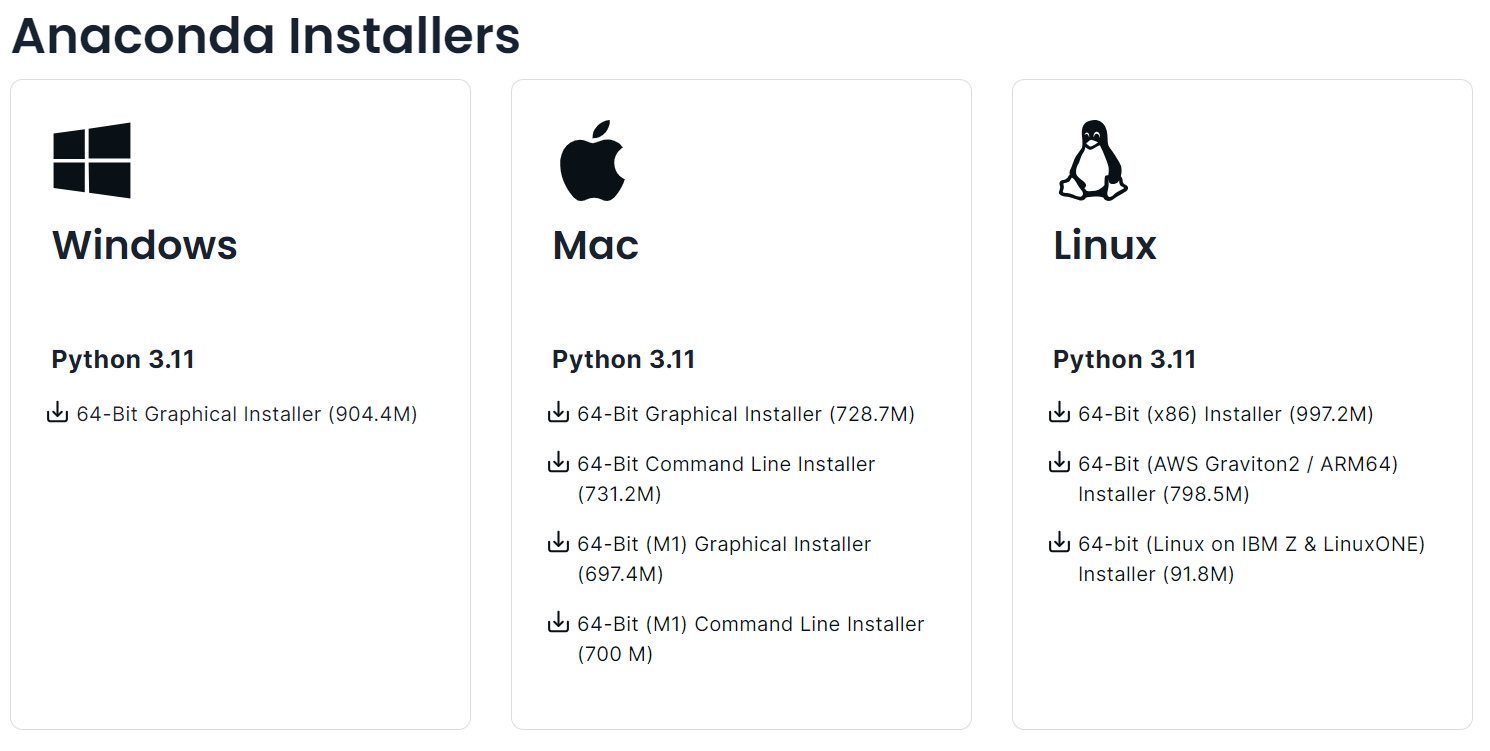
\includegraphics[width=0.99\textwidth]{img/sistema_operativo_anaconda.PNG}
        \caption{Instalación de anaconda según el sistema operativo. Fuente propia.}
        \label{fig:sistema_operativo_anaconda}
    \end{figure}
    \FloatBarrier
    
    Una vez descargado el instalador, se ejecuta y se siguen los pasos que se indican tales como la ubicación donde se desea guardar la aplicación, si se prefiere instalar solo para un usuario o para todos los que haya en el ordenador, etc. según lo que le interese a cada usuario. 
    
\subsubsection{2. Instalación del cuaderno de jupyter en anaconda}
    
    Al abrir la aplicación de anaconda en el sistema ``Anaconda Navigator'', no suele venir instalado el cuaderno de Jupyter Notebook, el cual se emplea para la realización del código por lo que, para instalarlo, se debe acceder al apartado de ``\textit{Home}'' de ``Anaconda Navigator'' y donde pone Jupyter Notebook se le da a ``install'' (si en lugar de poner ``install'', pone ``launch'' quiere decir que ya está instalado y, por tanto no se debe realizar este paso). La figura \ref{fig:instalacion_jupyterNotebook}, es un ejemplo donde el Jupyter Notebook ya está instado.

    \begin{figure}[ht]
        \centering
        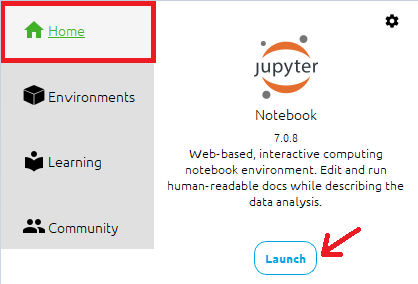
\includegraphics[width=0.70\textwidth]{img/instalacion_jupyterNotebook.PNG}
        \caption{Instalación de Jupyter Notebook realizada correctamente. Fuente propia.}
        \label{fig:instalacion_jupyterNotebook}
    \end{figure}
    \FloatBarrier

\subsubsection{3. Creación de un entorno para trabajar en este proyecto}
    
    La mejor forma de trabajar en Python sin sufrir problemas de versiones y bibliotecas es mediante entornos. Por eso, se emplea anaconda, ya que, permite crear un entorno distinto para cada trabajo que se realiza. De forma que, se pueden instalar diferentes versiones de Python y bibliotecas en los diferentes entornos, asegurando que los proyectos son independientes y no entran en conflicto. 

    Para instalar un nuevo entorno, se debe acceder al apartado ``\textit{Environments}'' de ``Anaconda Navigator'', ``\textit{Create}'', poner el nombre que se desee al entorno de trabajo con el que se va a trabajar y en packages seleccionar Python con la versión deseada tal y como se muestra en la figura \ref{fig:creacion_entorno}.
    
    \begin{figure}[h]
        \centering
        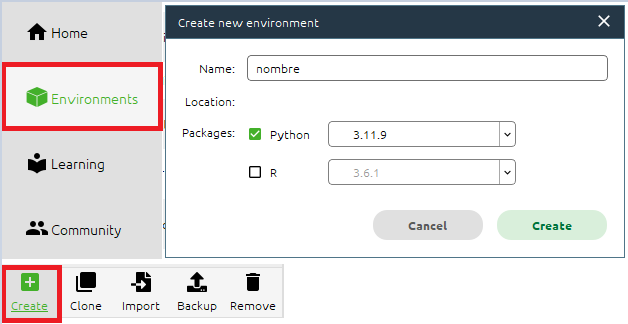
\includegraphics[width=0.99\textwidth]{img/creacion_entorno.PNG}
        \caption{Creación de un nuevo entorno en Anaconda Navigator. Fuente propia.}
        \label{fig:creacion_entorno}
    \end{figure}
    \FloatBarrier
    
    Pero, en este caso, al realizarlo de esta forma surgieron algunos problemas al instalar el paquete Tensorflow, imprescindible para este trabajo, por lo que, tras investigar en la página oficial de anaconda se decidió crear el entorno de una manera distinta. 
    
    Tal y como se indica en la página oficial de anaconda \footnote{\url{https://docs.anaconda.com/free/working-with-conda/applications/tensorflow/}}, una forma de crear un entorno con los paquetes de tensorflow instalados automáticamente es desde la consola de anaconda ``Anaconda Prompt'' a la cual se puede acceder desde el buscador de aplicaciones del sistema tal y como se muestra en la figura (Figura \ref{fig:acceso_consolaAnaconda}).
    
    \begin{figure}[h]
        \centering
        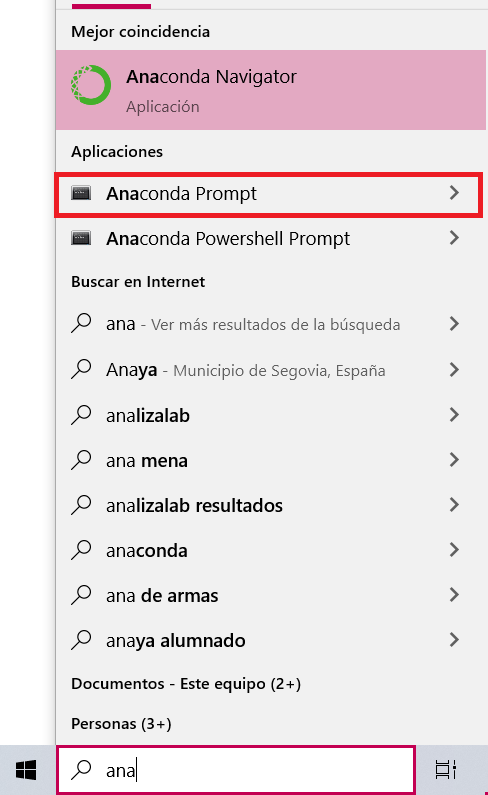
\includegraphics[width=0.60\textwidth]{img/acceso_consolaAnaconda.png}
        \caption{Acceso a la consola de ``Anaconda Prompt''. Fuente propia.}
        \label{fig:acceso_consolaAnaconda}
    \end{figure}
    \FloatBarrier
    
    En la consola de anaconda se debe escribir lo siguiente: ``\textit{conda create -n nombreEntorno tensorflow}'' para crear el entorno con los paquetes necesarios de Tensorflow instalados (Figura \ref{fig:nuevo_entorno}).
    
    \begin{figure}[h]
        \centering
        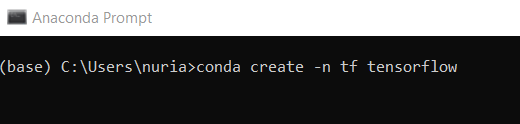
\includegraphics[width=0.99\textwidth]{img/nuevo_entorno.PNG}
        \caption{Creación de un nuevo entorno con Tensorflow con la consola de ``Anaconda Prompt''. Fuente propia.}
        \label{fig:nuevo_entorno}
    \end{figure}
   \FloatBarrier
    
    Una vez creado el entorno, para activarlo, se debe escribir lo siguiente en la consola ``Anaconda Prompt'': ``\textit{conda activate nombreEntorno}''.
    
    A la hora de trabajar con el entorno, se puede acceder tanto al cuaderno de jupyter (``Jupyter Notebook'') como a la consola de ese entorno especifico. Por lo general, se va a acceder al cuaderno de jupyter cada vez que se desee trabajar en el código pero, a la hora de instalar alguna biblioteca nueva o algún paquete necesario se hace a través de la consola (Figura \ref{fig:acceso_entorno}).
    
    \begin{figure}[h]
        \centering
        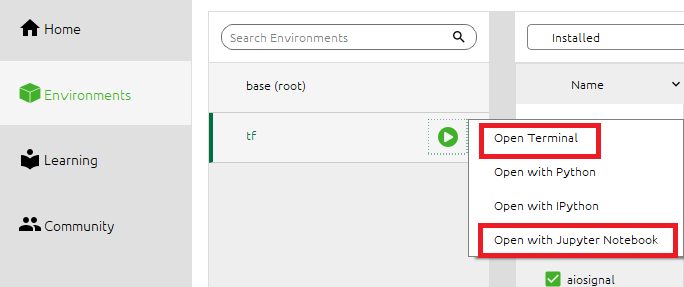
\includegraphics[width=0.99\textwidth]{img/acceso_entorno.png}
        \caption{Acceso a la terminal y Jupyter Notebook del entorno. Fuente propia.}
        \label{fig:acceso_entorno}
    \end{figure}
   \FloatBarrier

    Para instalar los paquetes necesarios bastará con poner en la consola \textit{``conda install nombrePaquete''}. Los paquetes extras que se deben tener instalados para este trabajo además de keras (el cual está dentro de Tensorflow y por lo tanto ya viene instalado con el entorno) son Numpy, Pandas y  Scikit-learn.
    
    Las versiones empleadas en este caso tanto de Python como de tensorflow han sido 3.10.13 y 2.10.0 respectivamente.
    

\section{Instalación / Puesta en marcha}

Una vez se tienen instalados los programas mencionados previamente, ya se puede acceder a los distintos \textit{notebooks} de Python y ejecutar las funciones realizadas para obtener todos los objetivos de este trabajo. Existen tres \textit{notebooks} distintos cuya función se explica a continuación.

\subsection{Carpeta ``data'' y ``data\_nuevo''}

Antes de explicar los distintos \textit{notebooks}, hay que destacar la carpeta ``\textit{data}'', en la cual se encuentran todas las imágenes empleadas para este trabajo y es fundamental para la ejecución de los siguientes \textit{notebooks}.

Dependiendo de donde se encuentre ubicada esta carpeta en el ordenador personal de cada usuario, se deberá cambiar la ruta asignada. Por ejemplo, en este caso, la carpeta se encuentra en la siguiente ruta: \textit{``C:/Users/nuria/Downloads/TFG''} y, por ende, la ruta nueva donde se creará la nueva carpeta con la nueva distribución de las imágenes (toda la explicación referida a esto se encuentra en el \textit{Anexo D}) será \textit{``C:/Users/nuria/Downloads/TFG/data\_nuevo''} en este caso ya que, en el código realizado se ha estipulado que la nueva carpeta se cree en el mismo directorio donde se encontraba la carpeta inicial.

\subsection{\textit{Notebook} ``redes neuronales - neumonía''}

Este es el \textit{notebook} principal con el que se ha trabajado desde un inicio. Incluye todas las funciones necesarias con su ejecución y su correspondiente explicación además de diversas aclaraciones a lo largo de todo el \textit{notebook}. Es el \textit{notebook} en el que se han basado los resultados explicados en la memoria.

Para ejecutar este \textit{notebook}, se han de seguir los siguientes pasos:

\begin{enumerate}
    \item En primer lugar, se han de ejecutar las funciones \textit{buscar\_imagen} y \textit{redestribucion\_imagenes} para obtener la carpeta \textit{data\_nuevo} a partir de la carpeta \textit{data} y, así poder trabajar con las imágenes correctamente distribuidas en las distintas subcarpetas tal y como se explica en el \textit{Anexo D}. 
    
    Hay que tener en cuenta que, con ejecutar esta función una vez, ya se deja creada la carpeta por lo que, no es necesario volver a ejecutarla en ningún otro momento.

    Tal y como se ha comentado previamente, a la hora de llamar a esta función, es necesario indicar el \textit{directorio\_principal} tal y como se muestra en la figura \ref{fig:llamar_funcion_redistrib_imagenes} y, este parámetro debe de ser modificado para cada usuario según donde se encuentre la carpeta \textit{data}.
    \begin{figure}[h]
        \centering
        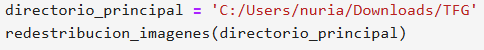
\includegraphics[width=0.99\textwidth]{img/llamar_funcion_redistrib_imagenes.PNG}
        \caption{Llamada a la función \textit{redestribucion\_imagenes} para este caso concreto. Fuente propia.}
        \label{fig:llamar_funcion_redistrib_imagenes}
    \end{figure}
    \FloatBarrier
    
    \item Posteriormente, se debe ejecutar la función \textit{preparar\_modelo} para configurar los generadores de datos para entrenar, validar y probar los modelos.
    \item A continuación, se ejecuta la función \textit{metricas} para calcular las distintas métricas que se van a emplear en la evaluación de los modelos.
    \item Después, se ejecutan las funciones \textit{establecer\_arquitectura\_propia} y \textit{establecer\_arquitectura\_AlexaNet} que establecen los distintos tipos de modelos de red neuronal para para la CNN propia y la de AlexNet que se van a comparar en las siguientes funciones.
    \item Luego, se ejecutan las funciones \textit{arq\_batch\_propia} y \textit{arq\_batch\_AlexNet} con las que se obtiene una tabla comparativa de las métricas calculadas en la función \textit{metricas} para los distintos modelos obtenidos de la función \textit{establecer\_arquitectura\_propia} o \textit{establecer\_arquitectura\_AlexaNet} y distintos valores de \textit{batch size} como son \textit{8, 16, 20, 32 y 64} tanto para la CNN propia como la CNN de AlexNet.

    En la figura \ref{fig:llamada_funcion_arq_batch_propia} se muestra la llamada a la función \textit{arq\_batch\_propia}. El parámetro \textit{ruta}, deberá ser modificado acorde a la ruta donde se encuentre la carpeta \textit{data\_nuevo} según el usuario, tal y como se ha comentado previamente. Los parámetros \textit{nombre\_carpeta\_hist}, \textit{nombre\_carpeta\_resultados} y \textit{nombre\_carpeta\_modelos} se corresponden con los nombres de las carpetas donde se guardan los históricos, los modelos y los resultados finales. En el notebook ``redes neuronales ejecucion archivo.py'' estos nombres son distintos debido a que los resultados que se guardan también lo son tal y como se explica posteriormente. El resto de parámetros son acordes a los modelos, \textit{batch size} y épocas que se han empleado en este trabajo.
    \begin{figure}[h]
        \centering
        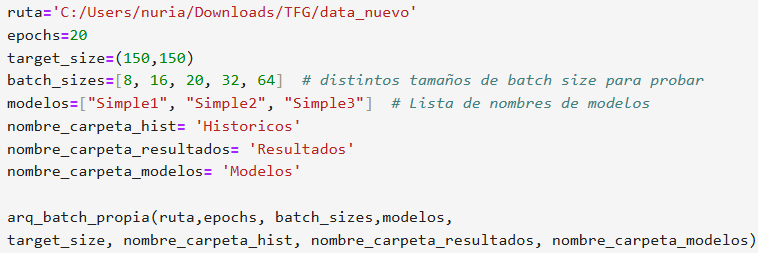
\includegraphics[width=0.99\textwidth]{img/llamada_funcion_arq_batch_propia.PNG}
        \caption{Llamada a la función \textit{arq\_batch\_propia} para este caso concreto. Fuente propia.}
        \label{fig:llamada_funcion_arq_batch_propia}
    \end{figure}
    \FloatBarrier
    \item Una vez se tienen las tablas comparativas de los distintos modelos y distintos \textit{batch size} tanto para la CNN propia como la CNN de AlexNet, ya se puede decidir qué CNN, modelo y \textit{batch size} consigue los mejores valores de métricas. Una vez escogido, se ejecuta la función \textit{neuronas} para el mejor modelo obtenido previamente (en este caso ha sido CNN AlexNet, modelo Simple3 y \textit{batch size} = 64). Con la función \textit{neuronas}, se obtiene una tabla comparativa de las métricas calculadas en la función \textit{metricas} para distintos valores de neuronas (\textit{512, 1024 y 2048}) en la capa oculta con el mejor modelo. A partir de aquí ya se puede determinar el mejor modelo final.

    La llamada a esta función se hace de manera similar a la figura \ref{fig:llamada_funcion_arq_batch_propia} pero con algunos cambios en los parámetros a tratar ya que, en este caso, no se usa como parámetro de entrada ni una lista de \textit{modelos} ni una lista de \textit{batch\_sizes} sino que, el \textit{batch\_size} es un número fijo el cual corresponde con el mejor modelo obtenido previamente. Además se añade un parámetro nuevo denominado \textit{num\_neuronas} que es una lista con los distintos valores de neuronas a probar en la capa oculta y el \textit{target\_size} en este caso es de (340, 340) ya que se emplea la CNN de AlexNet tal y como se puede apreciar en la figura \ref{fig:llamada_funcion_neuronas}.
    \begin{figure}[h]
        \centering
        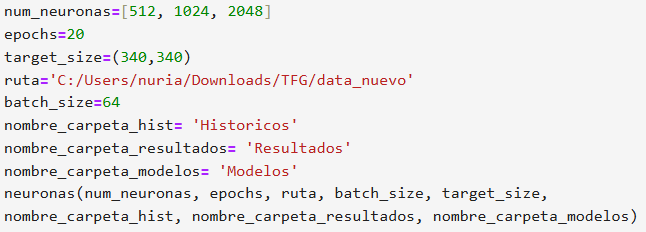
\includegraphics[width=0.99\textwidth]{img/llamada_funcion_neuronas.PNG}
        \caption{Llamada a la función \textit{neuronas} para este caso concreto. Fuente propia.}
        \label{fig:llamada_funcion_neuronas}
    \end{figure}
    \FloatBarrier
    \item Con el mejor modelo de red neuronal ya elegido para este caso, se pueden obtener gráficas para representar la evolución de dos métricas (loss o auc generalmente) durante el entrenamiento y la validación 
    del modelo, lo cual es útil para evaluar el rendimiento del modelo a lo largo de las épocas. Esto se consigue ejecutando la función \textit{grafica} y llamando a dicha función tal y como se muestra en la figura \ref{fig:grafica_auc} donde \textit{directorio\_historico} se refiere a la ruta donde se encuentra el archivo csv con las métricas del modelo del que se desea evaluar el rendimiento (modificar en caso de que la ruta a la carpeta ``Historicos'' sea modificada por el usuario). El parámetro \textit{metrica\_entrenamiento} es la métrica monitoreada durante el entrenamiento que se desea visualizar (en este caso es \textit{auc} aunque podría ser también \textit{loss} para ver el error) y, \textit{metrica\_validacion} se corresponde con la métrica monitoreada durante la validación que se desea visualizar (en este caso es \textit{val\_auc} pero, también podría ser \textit{val\_loss}). 
    \begin{figure}[h]
        \centering
        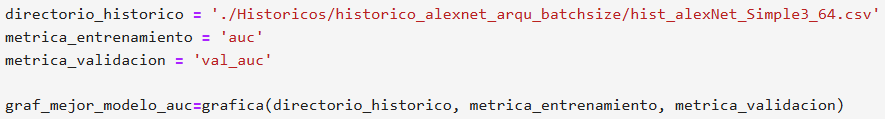
\includegraphics[width=0.99\textwidth]{img/grafica_auc.PNG}
        \caption{Llamada a la función \textit{grafica} con la métrica AUC. Fuente propia.}
        \label{fig:grafica_auc}
    \end{figure}
    \FloatBarrier
    \item Por último, se puede comparar el modelo más simple, (el cual se corresponde con el modelo Simple1 de la CNN propia) con el modelo final elegido por medio de sus matrices de confusión gracias a la función \textit{matriz\_conf}. La figura \ref{fig:llamar_funcion_matriz} muestra un ejemplo de cómo llamar a esta función para obtener la matriz de confusión del modelo más simple. El parámetro inicial \textit{ruta}, se corresponde con el directorio donde se encuentra la nueva carpeta creada con las imágenes \textit{data\_nuevo} y, deberá modificarse acorde a la ruta de esa carpeta para cada usuario. El parámetro \textit{modelo}, se refiere a la ruta donde se encuentra el archivo con el modelo que se desea emplear, en este caso, el modelo obtenido de la CNN propia, Simple1 y un \textit{batch size} de 8 (modificar en caso de que la ruta a la carpeta ``Modelos'' sea modificada por el usuario).
    \begin{figure}[h]
        \centering
        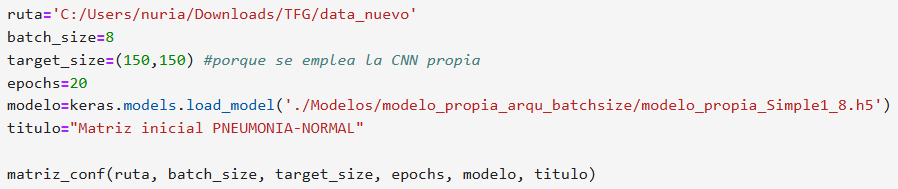
\includegraphics[width=0.99\textwidth]{img/llamar_funcion_matriz.PNG}
        \caption{Llamada a la función \textit{matriz\_conf} para obtener la matriz de confusión inicial. Fuente propia.}
        \label{fig:llamar_funcion_matriz}
    \end{figure}
\end{enumerate}
\FloatBarrier


Algo a tener en cuenta tanto en este \textit{notebook} como en el que se explica a continuación (``redes neuronales ejecucion archivo.py'') es que, en las funciones implementadas ``\textit{arq\_batch\_propia}'', ``\textit{arq\_batch\_AlexNet}'' y ``\textit{neuronas}'', se crean y se guardan dentro de una carpeta denominada ``Historicos'' o ``Historicos\_Py'' (según si se trata del primer \textit{notebook} o del segundo), distintos csv con las métricas obtenidas en el entrenamiento y la validación en cada bucle dependiendo de la función. Por ejemplo, a partir de este \textit{notebook}, en la función ``\textit{arq\_batch\_propia}'' se crea la carpeta ``Historicos'', con distintas subcarpetas, las cuales incluyen distintos ficheros csv para cada modelo y cada \textit{batch size}. A partir de estos csv, se puede crear posteriormente una gráfica para ver el rendimiento del modelo para el entrenamiento y la validación. 

En estas 3 funciones mencionadas previamente, también se crea una carpeta denominada ``Modelos'' con distintas subcarpetas donde se guardan los distintos modelos obtenidos tras el entrenamiento y una carpeta denominada ``Resultados'' con los \textit{dataframes} finales obtenidos para comparar las distintas métricas tras cada función. 

Las carpetas ``Historicos'', ``Modelos'' y ``Resultados'', están configuradas para crearse en el directorio actual, es decir, en la misma ruta en la que se encuentra el \textit{notebook} con el que se está trabajando y, solo en caso de no estar creadas ya. Si, por el contrario, el usuario prefiere guardar dichas carpetas en otro directorio, deberá modificar las tres funciones donde se crean las carpetas tal y como se explica a continuación.

Se va a poner el ejemplo con la función ``\textit{arq\_batch\_propia}'' y la carpeta de ``Historicos'' aunque, se realizaría de igual manera en las otras dos funciones y con las carpetas ``Modelos'' y ``Resultados''. 

En primer lugar, se ha de buscar la línea que pone \textit{ruta\_historicos = os.path.join('.', nombre\_carpeta\_hist)} en la función ``\textit{arq\_batch\_propia}'', donde se crea la ruta a la nueva carpeta de Historicos en el directorio actual. Para modificar esto y que, en lugar de crearse la ruta en el directorio actual se cree en otro directorio, bastará con modificar el punto \textit{'.'} por el directorio que se desee, por ejemplo \textit{``C:/Users/nuria/Downloads/TFG''} o, por el contrario, poner un nombre como puede ser \textit{directorio\_principal}, introducir este parámetro como parámetro inicial de la función y, a la hora de llamar a la función indicar que  \textit{directorio\_principal=``C:/Users/nuria/Downloads/TFG''}, tal y como se muestra en la figura \ref{fig:directorio_modelos_hist_result}. 

Hay que tener en cuenta que, en el caso de modificar alguna ruta, también habrá que modificar las rutas cuando se desea acceder a esas carpetas, por ejemplo, a la hora de llamar a la función \textit{grafica}, el parámetro de entrada \textit{directorio\_historico} tendrá que actualizarse a la nueva ruta y, lo mismo ocurre con la función \textit{matriz\_conf} y el parámetro \textit{modelo}.

\begin{figure}[h]
    \centering
    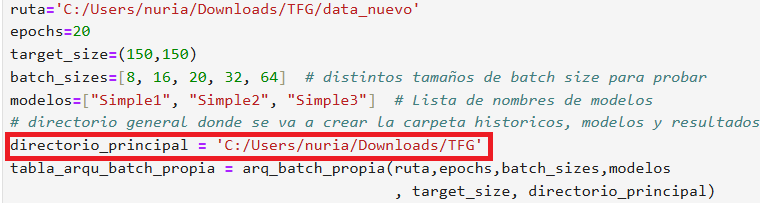
\includegraphics[width=0.99\textwidth]{img/direct_model_hist_result.png}
    \caption{Llamada a la función \textit{arq\_batch\_propia}. Fuente propia.}
    \label{fig:directorio_modelos_hist_result}
\end{figure}
\FloatBarrier


Otro punto a tener en cuenta es que, en este caso los mejores resultados se han obtenido para el modelo ``Simple3'' y, por tanto, la función \textit{neuronas} está configurada para este modelo, sin embargo, debido a la aleatoriedad de pesos y de muestras iniciales y a las similitudes en los resultados obtenidos en el modelo ``Simple2'' y ``Simple3'' explicado en el apartado de ``\textit{Resultados}'' de la memoria, en otra ejecución se puede obtener como mejor modelo el ``Simple2'' y la función \textit{neuronas} ya no serviría para este caso por lo que, a continuación se muestra qué habría que modificar en dicha función para adaptarlo a este modelo.

En la figura \ref{lst:neuronas_simple3} se muestra el fragmento de la función neuronas que deberá ser modificado. En este caso se corresponde con el modelo Simple3. En la figura \ref{lst:neuronas_simple2} se muestra el nuevo fragmento de código (perteneciente al modelo Simple2) que deberá ser sustituido por \ref{lst:neuronas_simple3} en la función \textit{neuronas}.

\begin{lstlisting}[caption={Segmento de la función neuronas correspondiente al modelo Simple3}, label={lst:neuronas_simple3}]
model = keras.Sequential(
            [
                keras.Input(shape=input_shape),
                layers.Conv2D(filters=96, kernel_size=(11,11), strides=(4,4), padding='valid', activation='relu'),
                layers.MaxPooling2D(pool_size=(3,3), strides=(2,2), padding='valid'),
                layers.BatchNormalization(),
                
                layers.Conv2D(filters=256, kernel_size=(5,5), strides=(1,1), padding='valid', activation='relu'),
                layers.MaxPooling2D(pool_size=(3,3), strides=(2,2), padding='valid'),
                layers.BatchNormalization(),
                
                layers.Conv2D(filters=384, kernel_size=(3,3), strides=(1,1), padding='valid', activation='relu'),
                layers.Conv2D(filters=384, kernel_size=(3,3), strides=(1,1), padding='valid', activation='relu'),
                layers.Conv2D(filters=256, kernel_size=(3,3), strides=(1,1), padding='valid', activation='relu'),
                layers.MaxPooling2D(pool_size=(3,3), strides=(2,2), padding='valid'),
                layers.BatchNormalization(),
                
                layers.Flatten(), 
                layers.Dense(neurona, activation='relu'), 
                layers.Dropout(0.2),
                layers.Dense(neurona, activation='relu'), 
                layers.Dropout(0.2),
                layers.Dense(1, activation='sigmoid'), 
            ]
        )
\end{lstlisting}


\begin{lstlisting}[caption={Segmento de la función neuronas correspondiente al modelo Simple2}, label={lst:neuronas_simple2}]
model = keras.Sequential(
            [
                keras.Input(shape=input_shape),
                layers.Conv2D(filters=96, kernel_size=(11,11), strides=(4,4), padding='valid', activation='relu'),
                layers.MaxPooling2D(pool_size=(3,3), strides=(2,2), padding='valid'),
                layers.BatchNormalization(),
                
                layers.Conv2D(filters=256, kernel_size=(5,5), strides=(1,1), padding='valid', activation='relu'),
                layers.MaxPooling2D(pool_size=(3,3), strides=(2,2), padding='valid'),
                layers.BatchNormalization(),
                
                layers.Conv2D(filters=384, kernel_size=(3,3), strides=(1,1), padding='valid', activation='relu'),
                layers.Conv2D(filters=384, kernel_size=(3,3), strides=(1,1), padding='valid', activation='relu'),
                layers.Conv2D(filters=256, kernel_size=(3,3), strides=(1,1), padding='valid', activation='relu'),
                layers.MaxPooling2D(pool_size=(3,3), strides=(2,2), padding='valid'),
                layers.BatchNormalization(),
                
                layers.Flatten(), 
                layers.Dense(neurona, activation='relu'), 
                layers.Dropout(0.2),
                layers.Dense(1, activation='sigmoid'), 
            ]
        )

\end{lstlisting}

\subsection{Archivo ``Funciones.py''} 

Un archivo <<.py>> es un archivo con código fuente de Python que se emplea para guardar scripts u otros archivos de Python. Es de gran utilidad para ejecutar las funciones desde cualquier computador ya que, los archivos <<.py>> pueden ser abiertos y editados desde cualquier editor de texto que contenga el intérprete Python \cite{onlineconvert24}.

Por lo tanto, el archivo ``Funciones.py'' incluye todas las funciones implementadas en el \textit{notebook} ``redes neuronales - neumonía'' para, poder ser ejecutadas desde cualquier editor de texto.

\subsection{\textit{Notebook} ``redes neuronales ejecucion archivo.py''} 

En este \textit{notebook} se muestra cómo importar y utilizar las funciones desde el archivo Funciones.py.

Por lo que se han vuelto a ejecutar todas las funciones del \textit{notebook} ``redes neuronales - neumonía'' pero esta vez, siendo importadas a partir del archivo <<.py>>.

Los resultados de las funciones en estos dos \textit{notebooks} pueden variar sutilmente ya que, como ya se ha comentado en el apartado de ``Resultados'' de la memoria, cada vez que se entrena el modelo, tanto los pesos iniciales como las muestras de entrenamiento se asignan de manera aleatoria por lo que los resultados pueden ser ligeramente distintos. Es por esto que, se han creado carpetas donde guardar los históricos, modelos y resultados específicas para este \textit{notebook} denominadas\textit{ Historicos\_Py}, \textit{Modelos\_Py} y \textit{Resultados\_Py}.


\section{Demostraciones prácticas}

Todas las demostraciones prácticas se encuentran correctamente explicadas y ejecutadas en cada uno de los \textit{notebooks} mencionados previamente.





    
     